\section{Matching Circuits and Tuners}
\label{sec:tuners}

% Transmission line theory (reflection, max power transfer)
% [1] Pozar pp 56--57
% [2] Ebert p 29
% [3] Pozar pp 77--78
From transmission line theory, it is known that the voltage and current waves present on a transmission line is composed of an incident and a reflected wave. The voltage and current at any distance, $z$, from the load are \cite{pozar2011microwave}:
\begin{align}
    V(z) &= V^+e^{-j\beta z} + V^-e^{j\beta z}\\
    I(z) &= \frac{V^+}{Z_0} e^{-j\beta z} - \frac{V^-}{Z_0} e^{j\beta z}
\end{align}
where
\begin{where}
\item[$V(z)$] Voltage at distance $z$ [\si{V}]
\item[$I(z)$] Current at distance $z$ [\si{A}]
\item[$V^+$] Amplitude of the incident wave [\si{V}]
\item[$V^-$] Amplitude of the reflected wave [\si{V}]
\item[$Z_0$] Characteristic impedance of the transmission line [\si{\ohm}]
\item[$z$] Distance from load to the considered point [\si{m}]
\item[$\beta$] The wave number $=2\pi/\lambda$ [\si{rad\per m}]
\end{where}
The load impedance is the voltage-to-current ratio where $z=0$,
\begin{equation}
    Z_L = \frac{V(0)}{I(0)} = \frac{V^+ + V^-}{V^+ - V^-}Z_0
\end{equation}
Solving this for $V^-$ yields
\begin{equation}
    V^- = \frac{Z_L - Z_0}{Z_L + Z_0} V^+
\end{equation}
The ratio between the reflected and incident wave is known as the \emph{reflection coefficient}, denoted $\Gamma$,
\begin{equation}
    \label{eq:reflect}
    \Gamma = \frac{V^-}{V^+} = \frac{Z_L-Z_0}{Z_L+Z_0}
\end{equation}
Generally, the reflection coefficient along a transmission line can be written as \cite{ebert1998transmission}
\begin{equation}
    \Gamma(z) = \Gamma e^{j2\beta z}
\end{equation}
Note that $\Gamma$ without parameters indicates $\Gamma(0)$.

\begin{figure}[htbp]
    \centering
    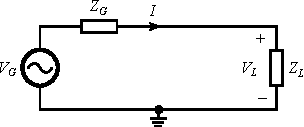
\includegraphics{img/analysis/generator_load}
    \caption{Equivalent circuit of a generator with given output impedance, $Z_G$, delivering power to a load of a given impedance, $Z_L$.}
    \label{fig:generator_load}
\end{figure}

The power in the load is found as \cite{pozar2011microwave}
\begin{equation}
    P = \frac{1}{2} \real{VI^*} = 
\end{equation}
where
\begin{where}
\item[$P$] Power delivered to the load
\item[$V$] Voltage drop across the load
\item[$I$] Current through the load
\end{where}

% Mismatch loss, S11. S11 = -6 dB  -->  SWR = 3

% Smith chart visualization

% Matching circuitry, L-network, smith chart ``ups and downs'', analytical formulas.

% Tuners: Series capacitor, shunt capacitor, variable inductor?

% Insertion loss, S21 for networks, equivalent series resistance, component Q.
